\documentclass[a4paper]{article}

\usepackage[czech]{babel} %https://github.com/michal-h21/biblatex-iso690
\usepackage[
   backend=biber      % if we want unicode 
  ,style=iso-numeric % or iso-numeric for numeric citation method          
  ,babel=other        % to support multiple languages in bibliography
  ,sortlocale=cs_CZ   % locale of main language, it is for sorting
  ,bibencoding=UTF8   % this is necessary only if bibliography file is in different encoding than main document
]{biblatex}

\usepackage[utf8]{inputenc}
\usepackage{fancyhdr}
\usepackage{amsmath}
\usepackage{amssymb}
\usepackage[left=2cm,right=2cm,top=2.5cm,bottom=2.5cm]{geometry}
\usepackage{graphicx}
\usepackage{pdfpages}
\usepackage{url}
\usepackage{multirow}
\usepackage{booktabs}
\usepackage{upgreek}

\usepackage{siunitx}
\sisetup{locale = DE}  %, separate-uncertainty = true    kdybych chtel +/-

\usepackage{float}
\newfloat{graph}{htbp}{grp}
\floatname{graph}{Graf}
\newfloat{tabulka}{htbp}{tbl}
\floatname{tabulka}{Tabulka}

\renewcommand{\thefootnote}{\roman{footnote}}

\pagestyle{fancy}
\lhead{PIV - (A3) Identifikace prvků na základě jejich charakteristického rentgenového záření}
\rhead{Vladislav Wohlrath}
\author{Vladislav Wohlrath}

\bibliography{source}

\begin{document}

\begin{titlepage}
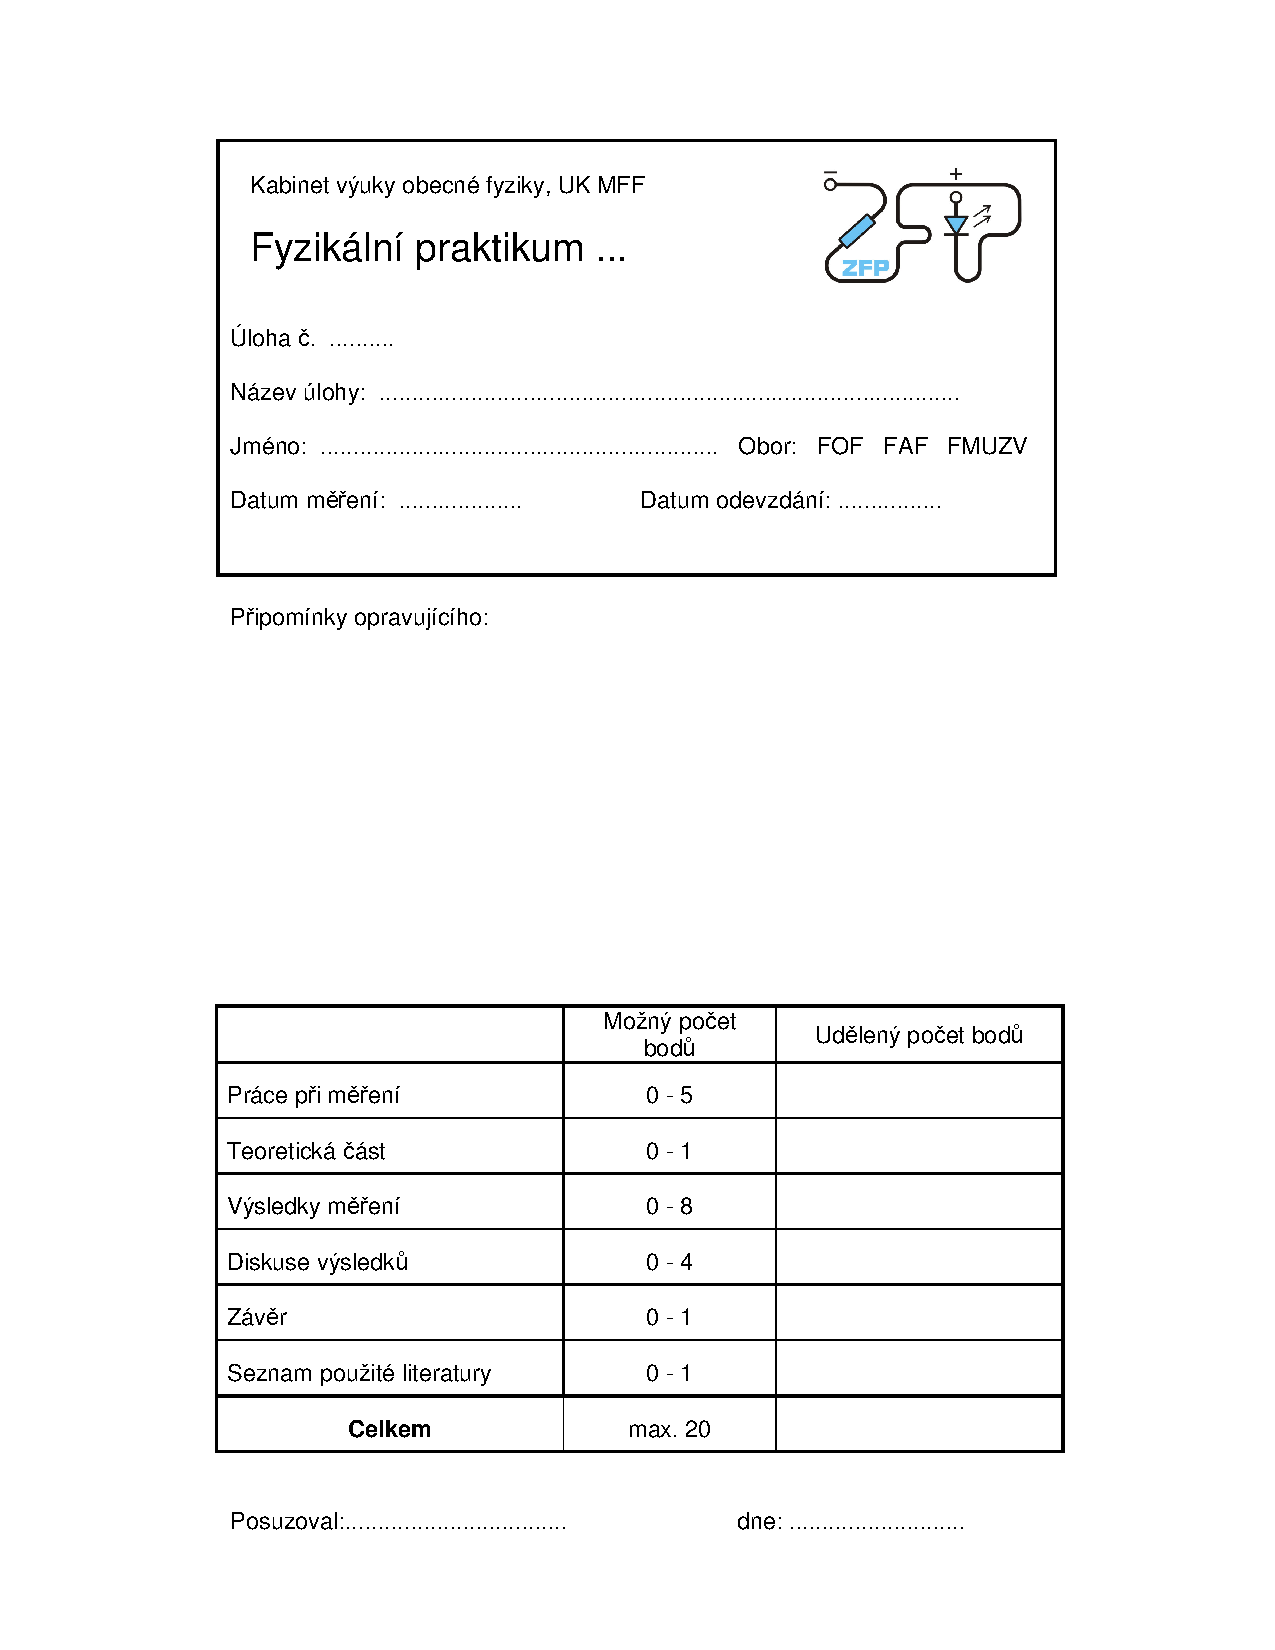
\includepdf[pages={1}]{./graficos/titlelist.pdf}
\end{titlepage}

\section*{Pracovní úkoly}
\begin{enumerate}
\item Proveďte energetickou kalibraci gama-spektrometru pomocí alfa-zářiče $^{241}$Am.
\item Určete materiál několika vzorků.
\item Stanovte závislost účinnosti výtěžku rentgenového záření na atomovém čísle elementu v daném experimentálním uspořádání.
\item Určete relativní zastoupení prvků v jednom ze vzorků.
\item Na základě rentgenového záření identifikujte radioaktivní vzorek a stanovte typ pozorovaného rozpadu.
\end{enumerate}

%Teoretická část
\section*{Teoretická část}

%Výsledky měření
\section*{Výsledky měření}
Nejprve jsme provedli energetickou kalibraci. Použili jsme tři známé peaky z gamma spektra $^{241}$Am: \SI{13.9}{\keV}, \SI{26.3}{\keV} a \SI{59.5}{\keV}. Další známý peak \SI{17.8}{\keV} jsme s novou kalibrací změřili na \SI{17.53}{\keV}, což nám dává představu o nejistotě měření energie.

Měřili jsme rentgenové spektrum celkem 7 čistých prvků a 2 dvouprvkových slitin. V tabulce \ref{t:merenivzorky} jsou uvedené naměřené energie pozorovaných přechodů a jejich výtěžek. Prvky jsme identifikovali podle přiložené tabulky energií charakteristického rentgenového záření.

U Cu jsme naměřili pouze jeden peak mezi K$\upalpha$ a K$\upbeta$, což odpovídá tomu, že jsou blízké a nedokážeme rozlišit. U všech ostatních prvků kromě Pb se nám podařilo rozlišit dva peaky, a to K$\upalpha$ a K$\upbeta$. U Pb jsme pozorovali pouze L$\upalpha$ a L$\upbeta$.

\begin{tabulka}[htbp]
\centering
\begin{tabular}{c||ccccc|c}
vzorek & energie (\si{\keV}) & FWHM (\si{\keV}) & net area & výtěžek (cps) & přechod & prvek \\ \hline\hline

1 & 8,17 & 1,16 & \num{24205(251)} & \num{30,3(3)} & K$\upalpha$ a K$\upbeta$ & $_{29}$Cu \\  \hline
\multirow{2}{*}{2} & 25,25 & 1,10 & \num{66467(331)} & \num{90,8(5)} & K$\upalpha$ & \multirow{2}{*}{$_{50}$Sn} \\
 & 28,58 & 1,08 & \num{14171(190)} & \num{19,4(3)} & K$\upbeta$ &  \\ \hline
\multirow{2}{*}{3} & 20,24 & 1,04 & \num{15116(171)} & \num{57,7(7)} & K$\upalpha$ & \multirow{2}{*}{$_{45}$Rh} \\ 
 & 22,84 & 0,96 & \num{3120(103)} & 10,9(4) & K$\upbeta$ & \\ \hline
\multirow{2}{*}{4} & 10,61 & 0,83 & \num{3556(112)} & 14,5(5) & L$\upalpha$ & \multirow{2}{*}{$_{82}$Pb} \\ 
 & 12,67 & 0,90 & \num{3823(123)} & 15,6(5) & L$\upbeta$ & \\ \hline
\multirow{2}{*}{11} & 23,16 & 1,02 & \num{17017(178)} & 83,4(9) & K$\upalpha$ & \multirow{2}{*}{$_{48}$Cd} \\ 
 & 26,18 & 1,15 & \num{4489(111)} & 22,0(6) & K$\upbeta$ & \\ \hline
\multirow{2}{*}{6} & 15,81 & 0,85 & \num{18116(249)} & 36,9(5) & K$\upalpha$ & \multirow{2}{*}{$_{40}$Zr} \\
 & 17,67 & 0,62 & \num{1639(126)} & 3,3(3) & K$\upbeta$ &  \\ \hline
\multirow{2}{*}{9} & 17,49 & 1,07 & \num{35230(274)} & 70,9(6) & K$\upalpha$ & \multirow{2}{*}{$_{42}$Mo} \\ 
 & 19,70 & 0,8 & \num{3881(143)} & 7,8(3) & K$\upbeta$ &  \\ \hline\hline
\multirow{3}{*}{5} & 8,43 & 1,28 & \num{3716(147)} & 5,5(2) & K$\upalpha$ a K$\upbeta$ & $_{29}$Cu \\
 & 22,15 & 1,02 & \num{23575(246)} & 34,7(4) & K$\upalpha$ & \multirow{2}{*}{$_{47}$Ag} \\
 & 25,03 & 1,03 & \num{7557(161)} & 11,2(3) & K$\upbeta$ & \\ \hline
\multirow{4}{*}{13} & 10,58 & 1,03 & \num{5293(129)} & 13,6(4) & L$\upalpha$ & \multirow{2}{*}{$_{82}$Pb} \\ 
 & 12,71 & 0,91 & \num{4834(148)} & 12,5(4) & L$\upbeta$ &  \\
 & 25,26 & 1,08 & \num{11483(158)} & 29,6(4) & K$\upalpha$ & \multirow{2}{*}{$_{50}$Sn} \\
 & 28,60 & 1,12 & \num{2958(94)} & 7,6(3) & K$\upbeta$ &  \\ 
\end{tabular}
\caption{Naměřené energetické přechody. V první části tabulky jsou čisté prvky, pod druhou tlustou čárou jsou slitiny.}
\label{t:merenivzorky}
\end{tabulka}

Graf závislosti výtěžku na protonovém čísle pro přechod K$\upalpha$ (který byl u všech prvků silnější než K$\upbeta$)je v grafu \ref{g:vytezek}.

\begin{graph}[htbp] 
\centering
%\input{graf.tex}
\caption{Závislost výtěžku na protonovém čísle pro přechod K$\upalpha$.}
\label{g:vytezek}
\end{graph}

%Diskuze výsledků
\section*{Diskuze}
Naměřené závislosti výtěžku na protonovém čísle dobře neodpovídá ani lineární ani kvadratický fit. Nicméně je zřejmý rostoucí trend, což souhlasí s \cite{skripta}. Kvadratický fit je samozřejmě pro nízká Z nepoužitelný. Pro interpolaci hodnot v měřeném rozsahu považujeme také lineární fit za lepší.

Pro jiné než K$\upalpha$ přechody jsme závislost nesestavovali, porovnávat výtěžky různých přechodů nemá význam.

Pokusili jsme se měřit ještě spektrum $_{26}$Fe, jenže kvůli nízkému protonovému číslu byl výtěžek příliš nízký pro určení spektrálních čar.

U Pb jsme určili, že se jedná o L přechody, především díky lehce rozpoznatelnému vzhledu olova a tomu, že druhý peak (s vyšší energií) nebyl výrazně slabší než ten první.

Nepřímo změřené relativní podíly u slitin 5 a 13 považujeme za poměrně nepřesné. Nejistotu jsme odhadli s ohledem na 

Mohlo se stát, že některý z peaků spektra vzorku se kryl s některým z peaků zářiče. V tom případě by byl výtěžek nadhodnocený. Stát se to mohlo především v okolí \SI{17.5}{\keV}, kde bylo možné naměřit až o \SI{6}{cps} více. 

%Závěr
\section*{Závěr}


\printbibliography[title={Seznam použité literatury}]

\end{document}